\section*{ТЕОРЕТИЧНІ ОСНОВИ ТА МЕТОДИ ДОСЛІДЖЕННЯ}

Методологічним підґрунтям дослідження є парадигма науки про проєктування (Design Science Research, DSR), яка зорієнтована на створення та оцінювання артефактів, що розв'язують практично значущі проблеми управління \cite{Hevner2004DSR}. Процедурну логіку побудови й оцінювання артефакту уточнено за методологією К.~Пефферса та співавторів \cite{Peffers2007DSRMeth}. У межах цієї парадигми артефактом виступає концептуальна модель і реалізований програмний механізм інтеграції генеративного штучного інтелекту (GenAI) та автономних агентів у процеси наукового адміністрування (research information management, RIM) закладу вищої освіти (ЗВО). Виклад побудовано як послідовність: концептуальна рамка переходу від реактивної до проактивної моделі управління $\rightarrow$ архітектура інтеграції GenAI $\rightarrow$ ядро механізму (золотий запис як конвеєр розв'язання сутностей) $\rightarrow$ дизайн відтворюваного оцінювання.

\subsection*{Реактивна та проактивна моделі управління науковою діяльністю}

Цифрова трансформація публічного та університетського управління — це не автоматизація наявних паперових процедур, а перепроєктування самих управлінських практик навколо даних \cite{Mergel2019DefiningDigitalTransformation}. Концепція цифрового врядування (digital-era governance) наголошує на реінтеграції розрізнених інформаційних потоків, переході до потребо-орієнтованої цілісності та цифровізації як організаційного, а не лише технічного зрушення \cite{Dunleavy2006DigitalEraGovernance}. Управління науковою інформацією (RIM) як окрема функція ЗВО систематизує дані про публікації, проєкти, авторів та результати для підтримки ухвалення рішень \cite{Bryant2017RIMDefining}.

Реактивна бібліометрична звітність працює за принципом \emph{post factum}: дані збирають уручну після завершення звітного періоду, верифікують і форматують під вимоги регулятора. Така модель має три системні вади. По-перше, висока трудомісткість: навіть консервативний сценарій малої або середньої кафедри передбачає кілька годин копіювання, звіряння та форматування, а опубліковані дослідження адміністративного навантаження науковців підтверджують, що звітні процедури є значною частиною дослідницького workflow \cite{Rockwell2009FDPBurden}. По-друге, фрагментація даних між незалежними джерелами (ORCID, Scopus, Web of Science, OpenAlex) породжує 15--25\,\% дублікатів у типових звітах. По-третє, реактивність позбавляє керівництво кафедри чи факультету можливості раннього втручання — рішення ухвалюють тоді, коли результат уже зафіксовано.

Проактивна модель управління науковою діяльністю натомість трактує наукометричні дані як безперервний керований потік. Інтегрований «золотий запис» дослідника й підрозділу оновлюється інкрементно, а керівник отримує доступ до актуальної картини в будь-який момент, а не лише наприкінці року. Це узгоджується з логікою євроінтеграції українського наукового простору: інфраструктури OpenAIRE та EOSC вимагають машиночитаних, інтероперабельних і безперервно підтримуваних даних \cite{OpenAIRE2023GuidelinesCRIS}, а модель RIM/CRIS описує організаційну роль таких даних у дослідницькому управлінні \cite{Bryant2017RIMDefining}. Стандарт CERIF, своєю чергою, задає канонічну схему сутностей наукової діяльності \cite{euroCRIS2024CERIF}. Перехід до проактивності — це передусім управлінське, а вже потім технічне завдання: змінюється не інструмент звітування, а сам цикл прийняття рішень.

\subsection*{Інженерна рамка TRACE: пошарова організація та ощадливість моделі}

Описане розмежування ролей систематизовано за інженерною рамкою \emph{TRACE}, призначеною для побудови довірених агентних систем у сферах з високою ціною помилки \cite{Zabolotnii2026TRACE}. Її засаднича теза --- довіра є властивістю \emph{архітектури}, а не окремої моделі, --- безпосередньо відповідає вимогам відповідального адміністрування. У термінах TRACE компоненти запропонованої системи розподіляються на чотири шари (рис.~\ref{fig:arch-trace}):

\begin{itemize}
    \item \textbf{L1 --- детерміноване ядро (trust anchor):} не-навчені, формально перевірювані правила --- канонізація DOI, жорсткі обмеження проти хибних злиттів (охоронець конфлікту DOI), фіксація провенансу;
    \item \textbf{L2a --- класичне машинне навчання:} парне логістичне зіставлення $\sigma(\boldsymbol{\beta}\cdot\boldsymbol{\phi})$ зі структурованими ознаками (відтворюване, з низькою латентністю);
    \item \textbf{L2b --- мовна модель як валідатор:} лише там, де потрібне розуміння природної мови (інтерпретація запиту, пояснення, перевірка узгодженості);
    \item \textbf{L3/L4 --- політика ескалації та нагляд людини:} смуга ручної перевірки (HITL) для невпевнених зіставлень і право оператора перевизначити будь-яке рішення.
\end{itemize}

\begin{figure}[ht]
\centering
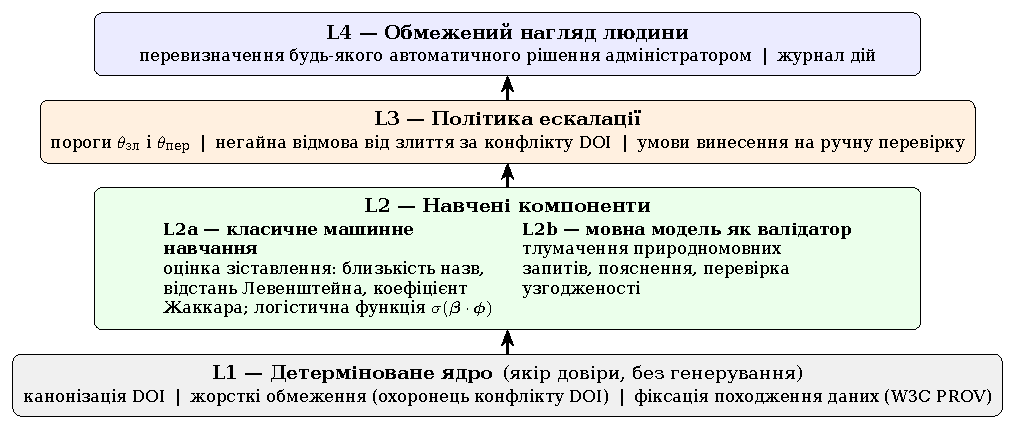
\includegraphics[width=0.95\linewidth]{../figures/arch_trace.pdf}
\caption{Чотиришарова архітектура запропонованої системи за інженерною рамкою TRACE: детерміноване ядро (L1) як якір довіри, інвентар навчених компонентів (L2a~--- класичний ML, L2b~--- LLM-валідатор), політика ескалації (L3) і обмежений нагляд людини (L4). Критичні для звітності операції виконує детермінований шар, а мовну модель застосовано лише там, де потрібне розуміння природної мови.}
\label{fig:arch-trace}
\end{figure}

Внутрішнім проєктним обмеженням рамки є \emph{ощадливість моделі} (Model Parsimony): тип навченого компонента обирається за відповідністю задачі, а не за презумпцією на користь LLM. Кількісним індикатором слугує коефіцієнт обчислювальної ощадливості (Computational Parsimony Ratio, CPR) --- відношення вартості найекономнішої адекватної моделі до вартості розгорнутої. Для ядра консолідації даних, реалізованого детерміновано (L1+L2a), $\mathrm{CPR}\approx 1$: система \emph{за побудовою} не витрачає мовну модель там, де достатньо детермінованих методів, що й робить її придатною для відповідального наукового адміністрування.

\subsection*{Функціональна архітектура ResearchIQ та агентний шар}

Ключовий ризик прямого застосування великих мовних моделей (LLM) в адмініструванні — фактичні галюцинації: моделі генерують правдоподібні, але хибні відомості \cite{Chelli2024HallucinationRates}, що неприпустимо для офіційної звітності. Тому ResearchIQ реалізує TRACE-поділ ролей: детерміноване ядро відповідає за критичні операції з даними, а GenAI використовується для інтерпретації запитів, пояснення результатів і гнучкого формування звітів \cite{Wang2024SurveyLLMAgents}.

ResearchIQ реалізовано як багатокористувацький вебзастосунок: React-інтерфейс забезпечує панель показників, список НПП, пошук ORCID, чат і генератор звітів; Node.js/Express API виконує автентифікацію, ізолює tenant-дані та проксіює запити до ORCID, OpenAlex і Scopus; серверний шар зберігає окремі JSON-набори для кожного ЗВО. Така будова відділяє презентаційний рівень від наукометричного конвеєра й дозволяє розгортати один застосунок для кількох закладів без змішування даних (рис.~\ref{fig:researchiq-app-arch}).

\begin{figure}[H]
\centering
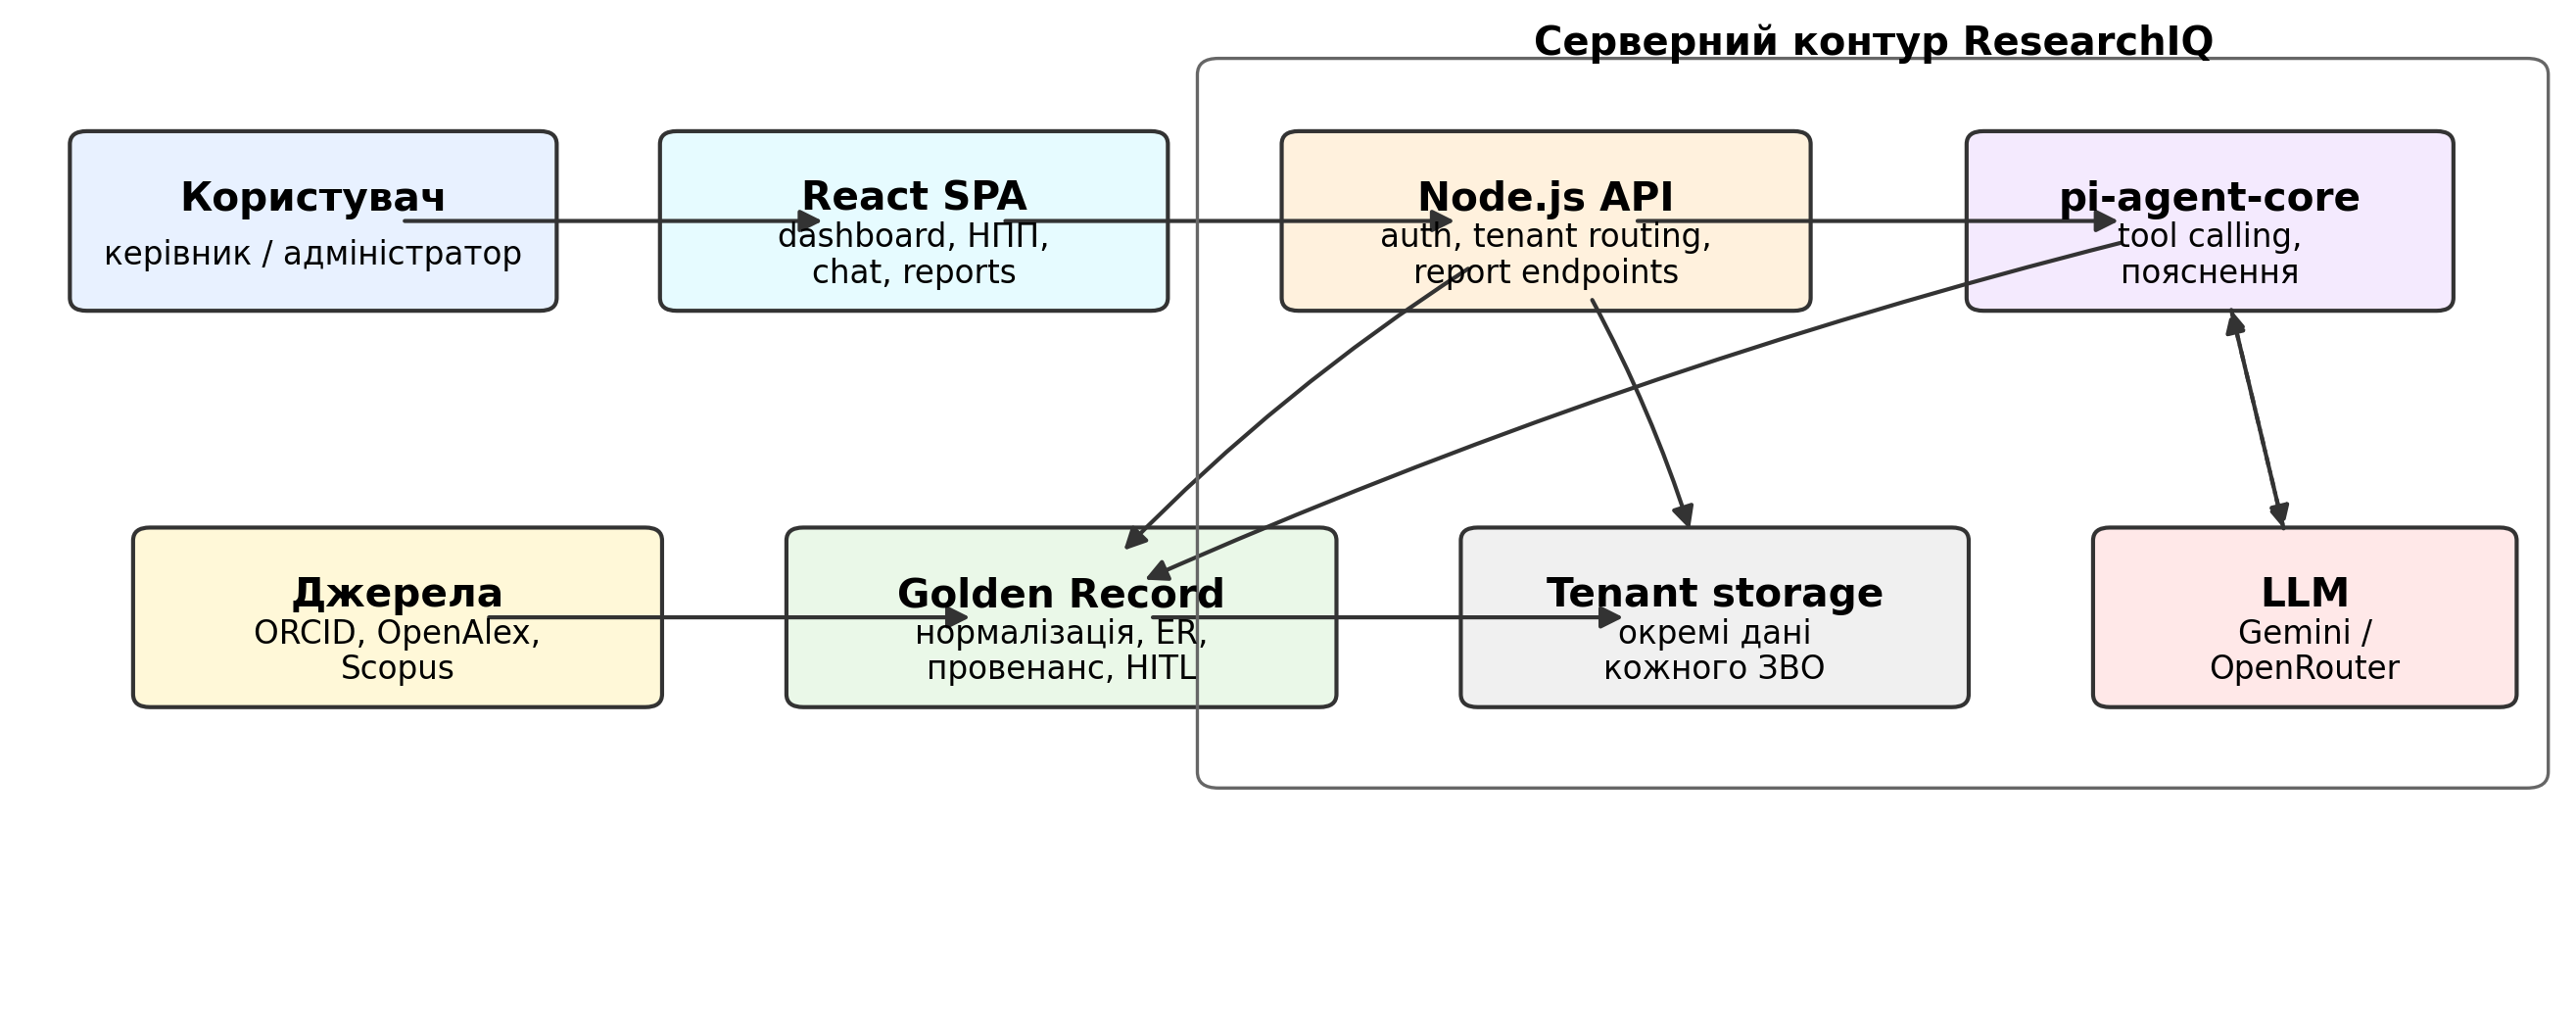
\includegraphics[width=0.95\linewidth]{../figures/researchiq_app_architecture.png}
\caption{Структурна схема ResearchIQ: користувацький інтерфейс, серверний API, tenant-сховище, конвеєр Golden Record, агентний шар на \texttt{pi-agent-core}, зовнішні наукометричні джерела та LLM-провайдери. Суцільні стрілки позначають потоки даних і детермінованих обчислень, пунктирні --- інтерпретаційні звернення агента до LLM.}
\label{fig:researchiq-app-arch}
\end{figure}

Агентний шар побудовано на \texttt{pi-agent-core}. Перед відповіддю агент отримує компактний знімок локальних даних ЗВО та реєстр типізованих інструментів: ранжування НПП за показниками, пошук локальних публікацій, порівняння кафедр, детальна картка науковця, оновлення метрик з OpenAlex, глобальний пошук праць, динаміка цитувань, мережа співпраці та поточна дата. Практична перевага GenAI у такій архітектурі полягає не в заміні обчислювального ядра, а в перетворенні складних аналітичних процедур на природномовний управлінський інтерфейс: керівник може ставити контекстні запитання, отримувати пояснення причин рейтингу чи ризику, швидко перебудовувати шаблон звіту під нову вимогу та бачити, з яких джерел походять показники. Це зменшує втрати часу на ручне переформатування й пошук потрібного зрізу даних, водночас зберігаючи перевірюваність результату.

Модель Gemini/OpenRouter, вибрана сервером, інтерпретує природномовний запит керівника і викликає потрібний інструмент, але відповідь спирається на обчислений результат, а не на вільну генерацію. Механізм функціональних викликів узгоджується з логікою MCP \cite{Anthropic2024MCP}: LLM планує, параметризує й пояснює, тоді як критичні операції збору, нормалізації, дедуплікації, злиття та побудови звітів виконує детермінований код. Отже, AI-агент у цій архітектурі є інтерфейсом управлінського запиту й оркестратором інструментів, а не джерелом бібліографічної істини.

\subsection*{Золотий запис як конвеєр розв'язання сутностей}

Ядром механізму є золотий запис (Golden Record) — конвеєр розв'язання сутностей (Entity Resolution, ER), що зводить розрізнені бібліографічні записи з різних джерел до єдиного канонічного представлення кожної публікації. Конвеєр складається з п'яти детермінованих кроків.

\emph{Крок 1. Канонізація сигнатури $\nu_\tau$.} Для кожного запису формується нормалізована сигнатура. Ідентифікатор DOI зводиться до нижнього регістру зі зняттям префіксів (\texttt{https://doi.org/}, \texttt{doi:}) та валідацією формату \texttt{10.x/...}; невалідні значення замінюються на \texttt{null}. Назва нормалізується за Unicode (NFKC, casefold) зі зняттям пунктуації через Unicode-клас, причому \emph{зі збереженням кирилиці}. Тут виправлено критичний дефект попереднього нормалізатора, який під час очищення пунктуації знищував усі кириличні символи, через що зіставлення за назвою для україномовних публікацій було повністю зламаним. Імена авторів проходять транслітерацію кирилиця$\rightarrow$латиниця для зведення варіантів написання (Заболотній С.~$\leftrightarrow$~Zabolotnii S.).

\emph{Крок 2. Блокування.} Щоб уникнути квадратичної складності $O(n^2)$ попарних порівнянь, кандидати на зіставлення групуються у блоки: за точним канонічним DOI; за двома найдовшими токенами назви; за парою «рік~$+$~токен». Порівнюються лише пари в межах спільного блоку.

\emph{Крок 3. Парне логістичне зіставлення.} Для пари записів обчислюється вектор ознак $\boldsymbol{\phi}$, а ймовірнісна оцінка тотожності визначається логістичною функцією:
\begin{equation}
\mathrm{score} = \sigma(\boldsymbol{\beta}\cdot\boldsymbol{\phi}) = \frac{1}{1+\exp\!\big(-\sum_{k}\beta_k\,\phi_k\big)},
\end{equation}
де $\sigma(\cdot)$ — сигмоїда, $\phi_k$ — значення $k$-ї ознаки, $\beta_k$ — її вага. Склад ознак і ваги наведено в табл.~\ref{tab:features}. Збіг DOI дає сильний позитивний внесок, а конфлікт DOI — сильний негативний, що відображає високу надійність цього ідентифікатора. Застосовано два пороги: $\theta_{\text{match}}=0{,}90$ для автоматичного злиття та $\theta_{\text{review}}=0{,}70$; пари зі значенням $\mathrm{score}\in[0{,}70;\,0{,}90)$ потрапляють у смугу ручної перевірки людиною (human-in-the-loop, HITL).

\begin{table}[ht]
\centering
\caption{Ознаки $\phi$ парного зіставлення та їхні ваги $\beta$}
\label{tab:features}
\begin{tabular}{lr}
\toprule
Ознака $\phi$ & Вага $\beta$ \\
\midrule
Збіг DOI (\texttt{doi\_match}) & $+3{,}0$ \\
Конфлікт DOI (\texttt{doi\_conflict}) & $-5{,}0$ \\
Косинусна близькість назв, TF (\texttt{title\_cosine}) & $+1{,}2$ \\
Символьна подібність, Левенштейн (\texttt{char\_sim}) & $+0{,}8$ \\
Узгодженість року, $|\Delta\text{рік}|\le 1$ (\texttt{year\_agree}) & $+0{,}6$ \\
Жаккар за журналом (\texttt{venue\_jaccard}) & $+0{,}4$ \\
Жаккар за авторами (\texttt{author\_jaccard}) & $+0{,}9$ \\
Збіг URL (\texttt{url\_match}) & $+0{,}2$ \\
\bottomrule
\end{tabular}
\end{table}

\emph{Крок 4. Кластеризація з охоронцем конфлікту DOI.} Записи, з'єднані ребрами зі $\mathrm{score}\ge\theta_{\text{match}}$, об'єднуються у зв'язні компоненти. Щоб запобігти хибним ланцюговим злиттям, застосовано охоронець: два кластери з непорожніми та неперетинними наборами валідних DOI не зливаються навіть за наявності транзитивного шляху між ними. Це блокує поширення помилки через проміжні неоднозначні записи.

\emph{Крок 5. Злиття атрибутів і провенанс.} Канонічний запис формується голосуванням, зваженим за надійністю джерела (Scopus/WoS $>$ OpenAlex $>$ ORCID); для лічильника цитувань береться максимум, для множин (автори, ключові слова) — об'єднання, для статусу відкритого доступу — оптимістичне рішення. Пріоритет джерел поля впорядковано як DOI~$\succ$~Crossref~$\succ$~CRIS~$\succ$~OpenAlex~$\succ$~ORCID. Кожне поле супроводжується провенансом у дусі W3C~PROV: фіксуються джерела, відповідність «поле~$\rightarrow$~джерело» та значення \texttt{matchScore}, що забезпечує повну простежуваність рішень для подальшого аудиту керівником.

\subsection*{Дизайн оцінювання}

Артефакт оцінюється на відтворюваному синтетичному бенчмарку, що моделює реалістичний український ЗВО (синтетичні дані, без реального закладу та персональних даних): 300 науково-педагогічних працівників, 20 кафедр (приблизно 5 факультетів). Кількість праць на дослідника задається лог-нормальним розподілом ($\mu=\ln 12$, $\sigma=0{,}9$) за період 2020--2024~рр.; розподіл дисциплін STEM~40\,\%~/ соціогуманітарні~35\,\%~/ медико-біологічні~25\,\% визначає ймовірність наявності DOI та мову публікації.

Кожна канонічна праця проєктується у записи ORCID, OpenAlex і Scopus із контрольованим дублюванням (цільова частка 15--25\,\%, базово 20\,\%) і спотворенням метаданих: транслітерація та переставлення авторів, відсутній або невалідний DOI («холодний» профіль ORCID втрачає DOI приблизно у 35\,\% випадків), зміна регістру та пунктуації, переклад назви (укр.~$\leftrightarrow$~англ.), абревіація журналу, зсув року на $\pm 1/\pm 2$, а також жорсткі негативи — колізії однакових назв із різними DOI. Інжектована карта дублікатів слугує gold-розміткою.

Якість оцінюється трьома групами метрик: парні Precision, Recall, F1; кластерна метрика B$^3$~F1 (Bagga--Baldwin); повнота й точність полів злитого запису. Базові методи й абляції застосовуються на ідентичних входах: DOI-only, Title$+$Year і повний Golden Record. Для статистичної надійності проведено симуляцію Монте-Карло з $K=30$ незалежними seed-ами; для кожної метрики наводиться середнє та 95\,\%-вий довірчий інтервал ($t$-інтервал). Додатково виконано розгортки за часткою дублікатів \{10, 15, 20, 25, 30\}\,\% та за множником спотворення \{0{,}25--2{,}0\}, що дозволяє оцінити чутливість методів до неоднорідності даних.
